\section{分运动论的初步知识}\label{sec:5-1}

分子运动论的基本内容是:
物质是由分子构成的;
分子永不停息地做无规则的运动;
分子之间有相互作用的引力和斥力。


\xiaobiaoti{分子}
在化学中已经学过,物质是由许许多多肉眼看不见的分子构成的,
分子是由原子构成的;
也有一些物质,如金属,是由原子直接构成的。

分子的体积非常小。
如果把分子看作是球形的,那么它的直径一般只有百亿分之几米。
百亿分之一米叫做埃(即 1 埃 $= 10^{-10}$ 米)。
因此,一般分子的直径大约是几个埃,例如,氧分子的直径大约是 3 埃。

由于分子非常小,所以通常物体里含有的分子数是非常多的。
在 0 ℃ 和 1 标准大气压下,$1\lflm$ 的气体里含有 $2.7 \times 10^{19}$ 个气体分子。
$1\lflm$ 的水里含有 $3.35 \times 10^{22}$ 个水分子。
为了帮助同学们想象这个数目有多大,设想把 $1\lflm$ 的水均匀地分布在整个地球的表面上,
那么每平方厘米还可以分得五千多个水分子。

\begin{wrapfigure}{r}{4cm}
    \centering
    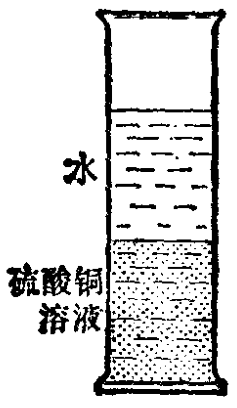
\includegraphics[width=3cm]{../pic/czwl2-ch5-1}
    \caption{}\label{fig:5-1}
\end{wrapfigure}

\xiaobiaoti{分子的运动}
组成物质的分子或原子(为了简单起见,以后我们只提分子)并不是静止不动的,而是在不停地运动着。
这可以从许多现象中看出来。
例如,一个空的瓶子(实际里边是空气)倒着放在装有红棕色二氧化氮气体的瓶子上,使两瓶口相对,
中间用玻璃片隔开,虽然二氧化氮比空气的密度大,但是当抽掉玻璃片以后,
可以看到红棕色的二氧化氮气体不断地向只有空气的瓶里运动,
最后两瓶气体的颜色变得完全相同,空气也运动到装二氧化氮的瓶里了。
这表明气体的分子是在不停地运动着。

象这样,不同的物质在互相接触时,彼此进入对方的现象叫做\textbf{扩散}。

扩散现象并不只是发生在气体之间,液体之间也有扩散现象。
在量筒里装半筒水,然后用长颈漏斗小心地把硫酸铜溶液倒进量筒的底部。
由于硫酸铜溶液比水的密度大,便沉在量筒的下部,和清水的界面非常清楚(图 \ref{fig:5-1})。
可是经过几天以后,蓝色的硫酸铜逐渐上升,界面变得模糊不清了。
再经过更长的时间,清水和硫酸铜溶液就混合均匀了。
这表明硫酸铜分子和水分子都在不停地运动。

固体之间也会发生扩散现象,只不过进行得很慢。
有人做过铅和金之间的扩散实验:将磨得很光滑的铅片和金片压在一起,
在室温下过了五年,结果铅片和金片便结合在一起了。
把它们切开后发现,铅和金相互渗透进去 1 毫米深。
可见,固体分子也在不停地运动。

大量实验表明,\CJKunderwave{一切物体里的分子都在不停地做无规则的运动}。

\begin{wrapfigure}{r}{4cm}
    \centering
    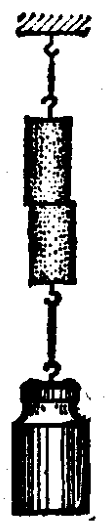
\includegraphics[width=1.5cm]{../pic/czwl2-ch5-2}
    \caption{分子引力实验}\label{fig:5-2}
\end{wrapfigure}

\xiaobiaoti{分子间的作用力}
既然物体是由分子组成的,而且分子在不停地运动着,那么,
为什么固体不会分散成一个一个的分子,而且能保持一定的体积和形状呢?
要把它的一部分跟另一部分分开,为什么比较困难呢?这是因为分子之间存在着引力的缘故。
当我们把物体的一部分跟另一部分分开时,就必须用力克服分子之间的引力。
把两块表面干净的铅压紧,由于分子间的引力,两块铅就结合在一起,
甚至在下面吊一个相当重的物体(图 \ref{fig:5-2}),也不能把它们拉开。

分子间还存在着互相排斥的力。这种斥力使分子间保持一定的间隙,而不是紧靠在一起。
固体和液体很难被压缩,就是由于分子间存在着斥力的缘故。

分子间的引力和斥力是同时存在的。
当分子间的引力和斥力相等时,分子处于平衡位置。
当分子间的距离十分靠近,小于平衡时的相互距离,斥力大于引力,分子间的作用力就表现为斥力。
当分子间的距离较大,大于平衡时的相互距离,引力大于斥力,分子间的作用力就表现为引力。
分子间的作用力随距离的增大而很快地减小。
当它们的距离大于分子直径的十倍以上时,分子间的作用力变得十分微弱,这时就常常近似地认为分子间没有作用力了。

